\documentclass[aspectratio=169]{beamer}

\usetheme{Madrid}
\usecolortheme{default}
\setbeamertemplate{navigation symbols}{}

\usepackage{lmodern}
\usepackage{graphicx}
\usepackage{booktabs}
\usepackage{amsmath}
\usepackage{hyperref}

\title{MAEG3080 Final Project}
\subtitle{CIFAR-100 Image Classification (SE-ResNet, PyTorch)}
\author{Student 1 \and Student 2 \and Student 3}
\institute{The Chinese University of Hong Kong}
\date{April 15, 2026}

\begin{document}

\begin{frame}
    \titlepage
\end{frame}

\begin{frame}{Project Objective}
    \begin{itemize}
        \item Train an image classifier on CIFAR-100 using PyTorch \emph{from scratch} (no pretrained weights)
        \item Use a compact \textbf{SE-ResNet} with squeeze-and-excitation blocks
        \item Two-stage pipeline: short baseline $\rightarrow$ finetune with RandAugment
        \item \textbf{Stage C:} further finetune from Stage~B with Mixup, CutMix, EMA (lower LR)
        \item Report official test accuracy using \texttt{results.py}
    \end{itemize}
\end{frame}

\begin{frame}{Dataset}
    \begin{itemize}
        \item CIFAR-100: 60,000 color images ($32 \times 32$)
        \item 100 fine-grained classes; 600 images per class
        \item 50,000 train / 10,000 test (official)
        \item Finetuning: 90\% train / 10\% stratified val (seed 42)
    \end{itemize}
\end{frame}

\begin{frame}{Model}
    \begin{itemize}
        \item SE-ResNet-style CNN (\texttt{se\_resnet}): residual blocks + SE attention
        \item Small configuration: base width 32; 2 blocks per stage
        \item Global average pooling $\rightarrow$ linear classifier (100 classes)
    \end{itemize}
\end{frame}

\begin{frame}{Training Pipeline}
    \begin{itemize}
        \item \textbf{Stage A:} 4 epochs, basic aug (crop, flip), SGD, $\sim$33\% test checkpoint
        \item \textbf{Stage B:} Load weights (\texttt{--init-from}), RandAugment, 30 epochs, lr 0.05
        \item \textbf{Stage C:} From Stage~B \texttt{best.pt}, 30 epochs, lr 0.015, warmup 3, batch 128
        \item Stage~C: Mixup/CutMix + RandAugment + EMA; script \texttt{iterate\_from\_stageb\_stage\_c\_mixema.sh}
        \item AMP on GPU; checkpoints on Google Drive (Colab); run name \texttt{sota\_se\_resnet\_exp1}
    \end{itemize}
\end{frame}

\begin{frame}{Implementation Workflow}
    \begin{enumerate}
        \item Train baseline (or reuse checkpoint) $\rightarrow$ \texttt{best.pt}
        \item Finetune with \texttt{iterate\_from\_34pct.sh} / quick script
        \item Evaluate with \texttt{results.py} on official test set
    \end{enumerate}
\end{frame}

\begin{frame}{Results (CIFAR-100)}
    \begin{table}
        \centering
        \begin{tabular}{ll}
            \toprule
            Setting & Accuracy \\
            \midrule
            Baseline (4 epochs, test eval) & $\approx 33.3\%$ \\
            Stage~B best val (epoch 28) & 65.22\% \\
            \textbf{Official test (Stage~B)} & \textbf{65.17\%} \\
            Stage~C best val (epoch 29) & 68.48\% \\
            \textbf{Official test (Stage~C)} & \textbf{68.14\%} \\
            \bottomrule
        \end{tabular}
    \end{table}
    \vspace{0.5em}
    \small Best row: \texttt{results.py} on Stage~C \texttt{sota\_se\_resnet\_exp1/best.pt}.
\end{frame}

\begin{frame}{Training curves (Colab run)}
    \centering
    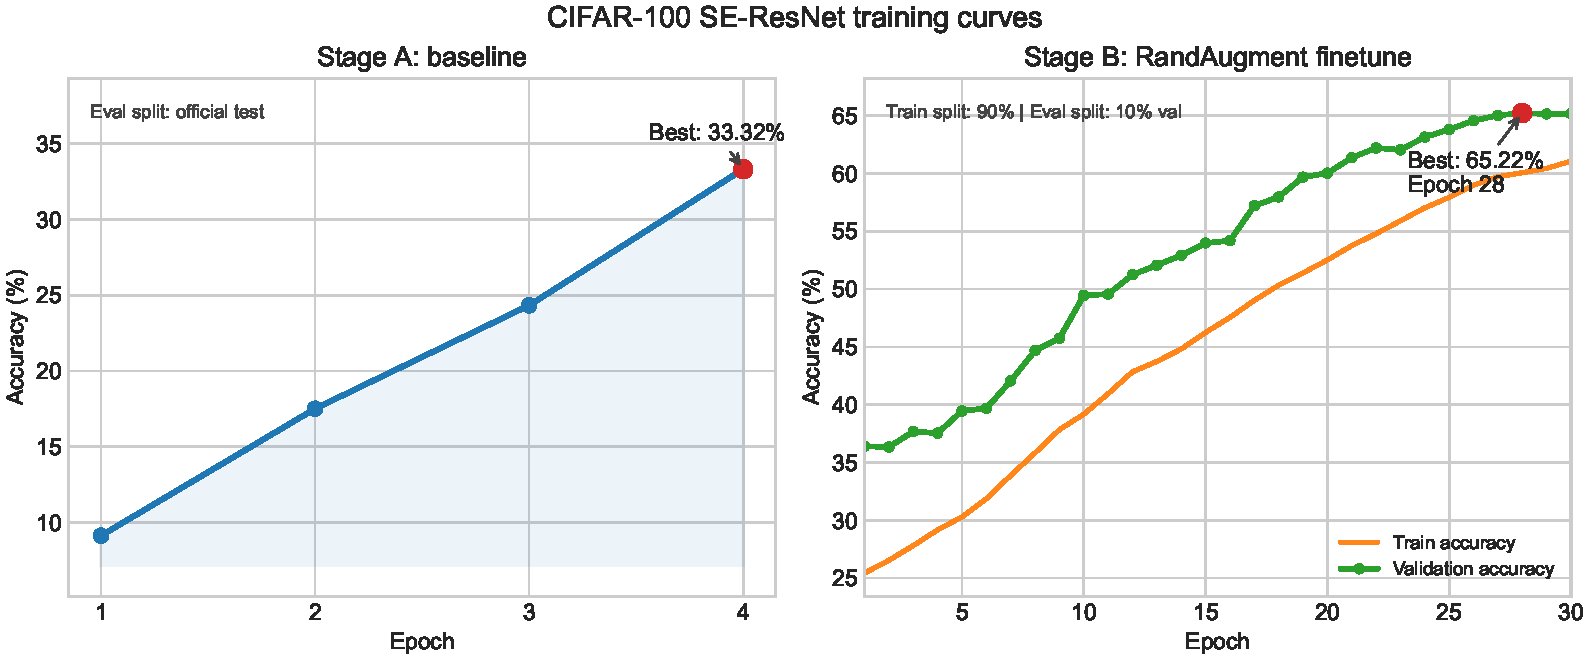
\includegraphics[width=0.92\linewidth]{../report/figures/training_curves_A_B.pdf}
    \vspace{0.3em}

    \small Left: Stage~A test accuracy; right: Stage~B train vs.\ val ($30$ epochs). Best val at epoch~28.
\end{frame}

\begin{frame}{What Worked}
    \begin{itemize}
        \item Initializing from a stable short baseline before strong augmentation
        \item RandAugment + longer finetune schedule on top of Stage~A ($\sim$65\% test)
        \item Stage~C: Mixup/CutMix + EMA finetune from Stage~B ($\sim$68\% test)
        \item Validation split for selection; official test only via \texttt{results.py}
    \end{itemize}
\end{frame}

\begin{frame}{Challenges}
    \begin{itemize}
        \item CIFAR-100 is hard: many similar classes, small images
        \item Large WRN / multi-hundred-epoch runs are costly on free Colab
        \item SE-ResNet path trades some ceiling for faster iteration and reliable gains
    \end{itemize}
\end{frame}

\begin{frame}{Group Contribution}
    \begin{itemize}
        \item Student 1: data preprocessing and augmentation experiments
        \item Student 2: model code, training pipeline, Colab workflow
        \item Student 3: result analysis, report writing, slides
    \end{itemize}
\end{frame}

\begin{frame}{Conclusion}
    \begin{itemize}
        \item SE-ResNet from scratch: baseline $\rightarrow$ Stage~B $\rightarrow$ Stage~C
        \item \textbf{68.14\%} official test (Stage~C); \textbf{65.17\%} after Stage~B only
        \item Independent \texttt{results.py} evaluation for final numbers
    \end{itemize}
\end{frame}

\begin{frame}
    \centering
    \Huge Questions?
\end{frame}

\end{document}
